\chapter{范畴语义}

本章介绍类型论的范畴语义. 注意我们研究类型论的
语义时, 类型论是被研究的数学对象, 而不是正在使用的数学语言.
此时使用的语言可以自由选择, 例如自然语言、集合论甚至类型论本身.
这个外部的语言称作\textbf{元语言}, 而被研究的类型论语言就直接
称作“语言”. 切忌混淆元语言中的概念与语言内的概念. 另一个
容易混淆的事情, 在于语义中的许多概念都是为了与语法中的事物
相对应, 因此二者会用相近的名称与记号, 但是它们也不应当混同.

类型论模型的一个极重要的特征就是其(广义的)代数性. 何为代数性?
最狭义来说, 一个代数结构就是某集合上配备一些运算, 并且满足
形如 \(\forall x_1, x_2, \dots, M = N\) 的公理. 例如
群、环、\(\Bbbk\)-向量空间等等. 代数结构通常满足一系列性质,
例如同态定理, 三条同构定理等. 对代数结构可以推广
得到\textbf{本质代数结构}或者\textbf{广义代数结构}. 而类型论
的模型一般都可以写成这种形式, 进而可以运用代数结构的一般结论.

历史上提出了很多描述类型论语义的方案. 为了使叙述更加清晰,
我们先介绍 Awodey 提出的自然模型~\cite{awodey:2018:natural},
再简单补充一些历史源流.
\cite{newstead:2018:natmod-poly} 也有较为详细的讲解.

\section{范畴与模型}

我们先来思考最类型论最直观的模型, 将类型解释为集合.
函数类型对应函数集合, 乘积类型对应乘积集合, 等等.
如果有依值类型 \(x{:}A \vdash B(x)\), 那么 \(B(x)\)
应当对应 “依值集合”, 也就是一族集合 \(Y_x\), 其中 \(x\)
取遍 \(A\) 所对应的集合.
不过, 在一般情况下, \(\Gamma \vdash B\) 依赖于语境
\(\Gamma\) 中的多个类型. 因此我们应该将语境解释为集合,
而类型解释为集合族. 如果 \(\Gamma\) 解释为集合 \(X\),
\(\Gamma \vdash B\) 解释为集合族 \(Y_{x \in X}\),
那么新语境 \(\Gamma, y{:}B\) 应该解释为集合族的不交并
\(\coprod_{x \in X} Y_x\).

这是定义依值类型论的模型时出现的一般现象. 我们先直观地认为
类型应该解释为某物, 而后对于依值类型我们提出对应的“依值某物”,
最后完整的解释是将语境对应为某物, 而类型对应于依值某物.

\berry{2}
一般来说, 这里提到的“某物”往往构成一个范畴, 并且许多语义上的
操作都对应范畴论中早有研究的概念, 因此便有了范畴语义的研究.
直觉上, 类型之间的箭头应该是函数. 但参考前文所说, 我们应当
考虑语境之间对应的箭头. 不难看出, 既然语境是一列类型
\(\Gamma = (x_1{:}A_1, \dots, x_n{:}A_n)\),
那么若 \(\Delta = (y_1{:}B_1, \dots, y_m{:}B_n)\),
则合适的箭头 \(\Gamma \to \Delta\) 应当是一列表达式
\((M_1, \dots, M_m)\), 使得 \(\Gamma \vdash M_k : B_k\).
对于 $m = n = 1$ 的情况, 这就与函数是一致的.
不过, 因为有依值类型, \(B_k\) 中可能用到了变量 \(y_1, \dots, y_{k-1}\).
这时候要将它们对应地替换成 \(M_1, \dots, M_{k-1}\).
我们将这列表达式 \(M_k\) 记作 \(\sigma\),
整体写作 \(\Gamma \vdash \sigma : \Delta\).
这些在 \ref{beginning:stlc:canonicity} 中已有提及,
\(\sigma\) 称作从 \(\Gamma\) 到 \(\Delta\) 的\textbf{代换}.

给定任何语境 \(\Gamma\), 我们应该有一个集合 \(\mathrm{Tp}(\Gamma)\),
表示这语境下合法的类型构成的集合. 如果再有一个代换
\(\Delta \vdash \sigma : \Gamma\), 那么就可以得到
函数 \(\mathrm{Tp}(\Gamma) \to \mathrm{Tp}(\Delta)\).
注意这里方向是相反的.
所有这些函数合在一起就构成了函子
\(\mathcal{C}\op \to \mathsf{Set}\), 也就是一个预层.
因此, 对于一般的模型来说, 我们也应当有一个范畴
\(\mathcal{C}\) 与其上的预层 \(\mathrm{Tp}\).

对于类型的元素来说, 有多种等价的提法.
其中最简单的办法是考虑某个语境中所有类型的元素的不交并
\(\mathrm{Tm}(\Gamma)\), 以及映射
\(\pi : \mathrm{Tm}(\Gamma) \to \mathrm{Tp}(\Gamma)\)
为每个元素赋予类型.
这就构成了两个预层之间的映射 \(\pi : \mathrm{Tm} \to \mathrm{Tp}\).
如果读者不喜欢将不同类型的元素放在同一个集合中, 之后会讨论
一些避免这种情况的等价的表述.

给定语境 \(\Gamma\) 与类型 \(A \in \mathrm{Tp}(\Gamma)\),\footnote{
需要时刻注意的是, 我们正在使用语法中的现象来启发语义的定义.
因此这里的“语境”既可以指语法中的一个具体的语境, 也可以指
其模型中的一个对象 \(\Gamma \in \mathcal{C}\).
以集合模型为例, 语法是能具体写出表达式的东西, 而语义中
这些则对应集合与集合之间的函数. 显然并不是所有集合都能写出
具体的表达式, 因此这两者需要区分.
} 我们应当能构造出语境 \(\Gamma, x{:}A\).
因为变量名无关紧要, 我们也写作 \((\Gamma, A)\).
正如范畴论中的大部分构造一样, 我们应当找出语法中它的泛性质,
并将其作为模型的定义中的一条需要满足的性质.

泛性质无非二者居其一: 描述从该对象出发的箭头有哪些,
或者描述指向该对象的箭头有哪些. \((\Gamma, A)\) 的泛性质是后者.
要构造 \(\Delta \to (\Gamma, A)\) 的代换,
就需要先构造 \(\Delta \to \Gamma\) 的代换 \(\sigma\),
再构造一个元素 \(\Delta \vdash t : A[\sigma]\).\berry{3}
换句话说, 这是说我们有一个拉回方
\[\begin{tikzcd}
{\hom(\Delta, (\Gamma, A))} & {\mathrm{Tm}(\Delta)} \\
{\hom(\Delta, \Gamma)} & {\mathrm{Tp}(\Delta)}
\arrow["\pi", from=1-2, to=2-2]
\arrow["{\sigma \mapsto A[\sigma]}"', from=2-1, to=2-2]
\arrow[from=1-1, to=2-1]
\arrow[from=1-1, to=1-2]
\arrow["\lrcorner"{anchor=center, pos=0.125}, draw=none, from=1-1, to=2-2]
\end{tikzcd}\]
这就完全定义了 \((\Gamma, A)\).
由于对每个 \(\Delta\) 都有这样的拉回方, 我们可以将其
综合为预层上的拉回操作. 这就得到了自然模型的定义.

\begin{comment}
\section{族与丛, 分类空间}

我们先从集合出发, 描述一个一般的现象.
假如我希望描述一族集合, 最直接的方法就是给定一个指标集 \(B\),
然后对每个 \(b \in B\), 指定一个集合 \(E_b\).
换句话说就是有 \(E_\bullet : B \to \mathsf{Set}\).
但是另一方面, 我也可以将所有的 \(E_b\) 聚合起来
成为一个大集合 \(E\), 再用一个函数 \(p : E \to B\) 指出
每个元素所属的指标 \(b\) 是哪一个. 这两种描述方式是等价的.

\begin{center}
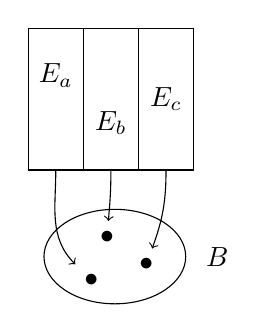
\begin{tikzpicture}
\draw (2,0) ellipse (0.9 and 0.6);
\node at (3.3,0) {\(B\)};
\node (C) at (2.4,-0.1) {\(\bullet\)};
\node (D) at (1.7,-0.3) {\(\bullet\)};
\node (E) at (1.9,0.25) {\(\bullet\)};

\draw (0.9,1.1) rectangle (1.6,2.9);
\node (Do) at (1.25, 2.3) {\(E_a\)};
\draw (1.6,1.1) rectangle (2.3,2.9);
\node (Eo) at (1.95, 1.7) {\(E_b\)};
\draw (2.3,1.1) rectangle (3,2.9);
\node (Co) at (2.65, 2) {\(E_c\)};
\draw (1.25,1.1) edge[->, out=-90] (D);
\draw (1.95,1.1) edge[->, out=-90, in=85] (E);
\draw (2.65,1.1) edge[->, out=-90, in=70] (C);
\end{tikzpicture}
\end{center}

事实上还有更加简单的例子. 考虑子集 \(E \subseteq B\).
它可以等价的描述为 \(B \to \{\cons{yes}, \cons{no}\}\),
因为只需要知道全集中的每个元素是否在这个子集里, 就完全确定了子集.
这是一种一般的现象, 即同一个概念可以描述为某种族 \(B \to U\),
也可以描述为某种丛 ------ 丛就是满足某条件的态射 \(p : E \to B\),
在子集的情况下就是单射 \(E \rightarrowtail B\),
而在集合族的情况下就是任何从集合到集合的映射.

下面的表格描述了数学中出现的许多族与丛的对应关系.
表格中画横线表示有这种构造, 但是没有通用的名字.
读者不必明白每个例子.

\begin{center}
\begin{tabular}{c c c c}\hline
族 & 族至丛 & 丛至族 & 丛\\\hline
\(\varphi : B \to \{\cons{yes}, \cons{no}\}\) &
\(E = \{b \in B \mid \varphi(b)\}\) &
\(\varphi(b) = (b \in E)\)&
子集 \(E \subseteq B\) \\
\(F : B \to \mathsf{Set}\) &
\!\!不交并 \(E = \coprod_{b} F(b)\)\!\! &
原象 \(F(b) = p^{-1}\{b\}\) &
\(p : E \to B\)\\
\(F : \mathcal C \to \mathsf{Set}\) &
元素范畴 \(\int^{\mathcal C}F\) &
原象 &
离散纤维化 \(\mathcal E \to \mathcal C\)\\
\!群同态 \(G \to \mathrm{Aut}(H)\)\!&
半直积 \(H \rtimes G\) &
------ &
分裂扩张 \(\hat G \to G\)\\
\(F : \mathcal C \to \mathsf{Cat}\) &
\!Grothendieck 构造\! &
原象 &
\!Grothendieck 纤维化\! \\
连续映射 \(B \to \mathbf{B}G\) &
------ &
分类映射 &
\(G\)-主丛 \(E \to B\)
\\\hline
\end{tabular}
\end{center}
\berry{2}

\(\{\cons{yes}\} \subseteq \{\cons{yes}, \cons{no}\}\)
可以看作是\textbf{万有}的子集, 因为对任何子集 \(E \subseteq B\),
以下交换方是拉回.
\[\begin{tikzcd}
  E & {\{\cons{yes}\}} \\
  B & {\{\cons{yes}, \cons{no}\}}
  \arrow[hook, from=1-1, to=2-1]
  \arrow[hook, from=1-2, to=2-2]
  \arrow[from=1-1, to=1-2]
  \arrow[from=2-1, to=2-2]
  \arrow["\lrcorner"{anchor=center, pos=0.125}, draw=none, from=1-1, to=2-2]
\end{tikzcd}\]
从这个角度看, 一切子集都源于
\(\{\cons{yes}\} \subseteq \{\cons{yes}, \cons{no}\}\),
或者说, 这个子集包含了一切其他子集可能出现的情况.
更严格来说, 有如下性质.
\begin{theorem}
对于集合 \(B\), 它的子集与映射 \(B \to \{\cons{yes}, \cons{no}\}\)
一一对应, 并且对应关系是上图的拉回关系.
\end{theorem}
因此, 我们说 \(\{\cons{yes}\} \subseteq \{\cons{yes}, \cons{no}\}\)
\textbf{分类}了全体子集.
这可以类推到集合族上.
考虑 \(\mathsf{Set}_*\) 为全体形如
\((A, a)\) 的有序对, 其中 \(a \in A\).%
\footnote{这里为了避免处理真类的问题, 可以不考虑全体集合.
例如可以固定一个较大的集合 \(U\), 只考虑这个集合的子集.}
有显然的映射 \(\mathsf{Set}_* \to \mathsf{Set}\),
将 \((A, a)\) 映射到 \(A\).
这样, 如果有集合族 \(E_\bullet : B \to \mathsf{Set}\),
那么也不难验证这是拉回.
\[\begin{tikzcd}
  E & {\mathsf{Set}_*} \\
  B & {\mathsf{Set}}
  \arrow[from=1-1, to=2-1]
  \arrow[from=1-2, to=2-2]
  \arrow[from=1-1, to=1-2]
  \arrow["{E_\bullet}"', from=2-1, to=2-2]
  \arrow["\lrcorner"{anchor=center, pos=0.125}, draw=none, from=1-1, to=2-2]
\end{tikzcd}\]
类似地可以说 \(\mathsf{Set}_* \to \mathsf{Set}\) 分类了全体集合族.

当然, 上面的说法有一些不严谨, 因为两个不同的 \(E_\bullet\)
可能给出同构的 \(E \to B\). 因为态射之间是直接比较相等,
而对象之间比较的是同构的概念, 这种情况难免出现.
子集能避免这个问题, 是因为两个子集之间至多有一种方法同构.
如果有 \(X_* \to X\), 使得在 \(E \to B\) 与某个
\(B \to X\) 之间有拉回的对应关系,
不过多个 \(B \to X\) 可能对应同构的 \(E \to B\),
就称 \(X_* \to X\) \textbf{弱分类}了 \(E \to B\) 的态射.
\end{comment}

\section{类型论的自然模型}\label{category:naturalmodel}
\begin{definition}\label{category:naturalmodeldef}
一个\textbf{自然模型}是任意一个有终对象的范畴 \(\mathcal C\),
配备两个预层与其间的态射 \(\pi : \mathrm{Tm} \to \mathrm{Tp}\),
使得对于任何 \(\Gamma \in \mathcal C\)
与 \(A \in \mathrm{Tp}(\Gamma) \cong \hom(\yo(\Gamma), \mathrm{Tp})\),
有对象表出以下拉回预层:
\[\begin{tikzcd}
\bullet & {\mathrm{Tm}} \\
{\yo(\Gamma)} & {\mathrm{Tp}}
\arrow["\pi", from=1-2, to=2-2]
\arrow["A"', from=2-1, to=2-2]
\arrow[from=1-1, to=2-1]
\arrow[from=1-1, to=1-2]
\arrow["\lrcorner"{anchor=center, pos=0.125}, draw=none, from=1-1, to=2-2]
\end{tikzcd}\]
此对象记作 \((\Gamma, A)\). 满足这种条件的态射也称作\textbf{可表态射}.
另外, 将态射 \((\Gamma, A) \to \Gamma\) 记作 \(\cons{p}_A\),
交换图上沿的态射记作 \(\cons{q}_A\).
\end{definition}

考虑所有合法语境在判值相等关系下构成的集合 \(\mathcal C\),
两个语境之间的态射 \(\sigma \in \hom(\Delta, \Gamma)\) 是代换,
% 即一列类型与 \(\Gamma\) 相符的表达式, 其中包含 \(\Delta\) 的变量.
判值相等的代换视为相同, 这样就构成一个范畴. 终对象是空语境.
对于每个语境 \(\Gamma\),
考虑允许包含 \(\Gamma\) 中的变量的合法的类型构成的集合 \(\mathrm{Tp}(\Gamma)\),
同样将判值相等的类型视为相同.
这些类型的元素的不交并记作 \(\mathrm{Tm}(\Gamma)\).
这样, 如果 \(\Gamma\) 下 \(A\) 是合法的类型,
又有代换 \(\sigma \in \hom(\Delta, \Gamma)\),
那么就可以将 \(A\) 中的变量代换得到 \(A[\sigma]\),
是 \(\Delta\) 下合法的类型.
这就证明了 \(\mathrm{Tp}\) 是预层. 同理 \(\mathrm{Tm}\) 也是预层.
\(\pi\) 将每个 \(a \in \mathrm{Tm}(\Gamma)\) 映射到它所属的类型.

我们来计算定义中提到的拉回. 我们知道预层的拉回是逐点计算的,
因此拉回 \(F\) 满足
\begin{align*}
F(\Delta)
&\cong \hom(\Delta, \Gamma) \times_{\mathrm{Tp}(\Delta)} \mathrm{Tm}(\Delta)\\
&= \{(\sigma, a) \mid \pi(a) = A[\sigma]\}\\
&= \hom(\Delta, (\Gamma, A)).
\end{align*}
因此 \(F\) 的确可表, 并且其表出对象就对应语境的扩展操作 \((\Gamma, A)\).

以上就证明了类型论的语法范畴构成自然模型, 记作 \(\mathbf T\).%
\footnote{当然, 因为我们还没有引入任何类型, 语法范畴其实是平凡的.
但是上面的证明可以随着加入新的类型而随时拓展.}
以此为模板, 就可以找到类型论语法中许多概念的语义对应.
例如, 类型论中的语境对应自然模型中 \(\mathcal C\) 的对象,
语境之间的代换对应 \(\mathcal C\) 中的态射.
语境中的类型对应 \(\mathrm{Tp}(\Gamma)\) 的元素.
给定 \(A : \mathrm{Tp}(\Gamma)\),
类型论中 \(A\) 的元素对应模型中的
\[\{a \mid a \in \mathrm{Tm}(\Gamma), \pi(a) = A\}.\]
由拉回的性质, 可以看出这等价于
\[\{\alpha \mid \alpha \in \hom(\Gamma, (\Gamma, A)), \cons{p}_A \circ \alpha = \cons{id}_\Gamma\}.\]
对于 \(A : \mathrm{Tp}(\Gamma), \sigma : \Delta \to \Gamma\),
由于 \(\mathrm{Tp}\) 是预层, 我们可以得到 \(A[\sigma] : \mathrm{Tp}(\Delta)\).
这是类型论中代换的对应. 而由于下图中右侧的正方形与外侧的正方形均是拉回,
\[\begin{tikzcd}
  {\yo(\Delta, A[\sigma])} & {\yo(\Gamma,A)} & {\mathrm{Tm}} \\
  {\yo(\Delta)} & {\yo(\Gamma)} & {\mathrm{Tp}}
  \arrow[from=2-2, to=2-3]
  \arrow[from=1-3, to=2-3]
  \arrow[from=1-2, to=2-2]
  \arrow[from=1-2, to=1-3]
  \arrow[from=2-1, to=2-2]
  \arrow[from=1-1, to=2-1]
  \arrow[curve={height=-9pt}, from=1-1, to=1-3]
  \arrow[dashed, from=1-1, to=1-2]
\end{tikzcd}\]
我们得到虚线的箭头也存在, 使得整体构成交换图并且左侧的正方形是拉回.
因此在 \(\mathcal C\) 中有这样一个拉回.
\[\begin{tikzcd}
  {(\Delta, A[\sigma])} & {(\Gamma,A)} \\
  \Delta & \Gamma
  \arrow[from=1-2, to=2-2]
  \arrow[from=2-1, to=2-2]
  \arrow[from=1-1, to=2-1]
  \arrow[dashed, from=1-1, to=1-2]
\end{tikzcd}\]
在一些其他的类型论的模型的定义中,
不涉及预层范畴, 而是直接将这个拉回作为类型论中代换的定义.

如何说明自然模型的确是合适的概念呢?
模型最重要的作用, 是语法中的概念可以解释到所有模型中.
用范畴的语言来说, 对于任何模型 \(\mathbf M\),
都有唯一的保持结构的态射 \(\mathbf T \to \mathbf M\).
这一点可以靠对语法归纳来证明.
我们之后会定义带有 \(\Pi\)-类型的模型, 带有 \(\Sigma\)-类型的模型, 等等.
它们各自也有对应的性质:
考虑带有 \(\Pi\)-类型的类型论构成的语法模型,
它到任何带有 \(\Pi\)-类型的模型都有唯一的保持结构的态射,
以此类推.

上面还没有定义何为保持结构的态射.
以下为了方便, 对于模型 \(\mathbf M\),
记它对应的范畴为 \(\mathcal C_{\mathbf M}\),
配备的预层是 \(\mathrm{Tm}_{\mathbf M}, \mathrm{Tp}_{\mathbf M}\),
有可表态射 \(\pi_{\mathbf M}\).
假如有函子 \(F : \mathcal C \to \mathcal D\),
那么复合上这个函子, 就给出了预层范畴之间的映射
\(F^* : \mathsf{Psh}(\mathcal D) \to \mathsf{Psh}(\mathcal C)\).

\begin{definition}
给定两个自然模型 \(\mathbf M, \mathbf N\),
定义一个\textbf{态射} \(F : \mathbf M \to \mathbf N\) 为
一个函子 \(F : \mathcal C_{\mathbf M} \to \mathcal C_{\mathbf N}\),
两个态射 \(F_{\mathrm{Tp}} , F_{\mathrm{Tm}}\) 使得以下图表交换:
\[\begin{tikzcd}
  {\mathrm{Tm}_{\mathbf M}} & {F^*\mathrm{Tm}_{\mathbf N}} \\
  {\mathrm{Tp}_{\mathbf M}} & {F^*\mathrm{Tp}_{\mathbf N}}
  \arrow["{F_{\mathrm{Tp}}}"', from=2-1, to=2-2]
  \arrow["{F_{\mathrm{Tm}}}", from=1-1, to=1-2]
  \arrow["{\pi_{\mathbf M}}"', from=1-1, to=2-1]
  \arrow["{F^* \pi_{\mathbf N}}", from=1-2, to=2-2]
\end{tikzcd}\]
此时对于任何 \(\Gamma \in \mathcal C_{\mathbf M}\) 与
\(A \in \mathrm{Tp}_{\mathbf M}(\Gamma)\), 有
\(F(\Gamma) \in \mathcal C_{\mathbf N}\) 与
\(F_{\mathrm{Tp}}(A) \in \mathrm{Tp}_{\mathbf N}(F(\Gamma))\),
并且自然诱导一个态射 \(F(\Gamma, A) \to (F(\Gamma), F_{\mathrm{Tp}}(A))\).
我们要求这个态射是同构.
\end{definition}

其中, 最后这个条件是在要求自然模型之间的态射保持 \((-,-)\) 这个运算.
如果这不仅是同构, 而是直接严格相等, 就说\(F\)是自然模型之间的\textbf{严格态射}.

\subsection{自然模型中的类型}

自然模型仅仅是搭建起了类型论模型的基本框架.
接下来, 我们要为这个框架加入具体的类型.
先从最简单的单元素类型开始.

我们同样从语法范畴寻找启发. 对于有单元素类型的类型论,
在任何语境 \(\Gamma\) 下都有 \(\Gamma \vdash \cons{Unit}\,\text{type}\).
因此应当有预层的态射 \(1 \to \mathrm{Tp}\),
在 \(\mathrm{Tp}\) 中指出单位类型.
而单位类型在任何语境下都恰好有一个元素. 因此如果考虑拉回
\[\begin{tikzcd}
  \bullet & {\mathrm{Tm}} \\
  1 & {\mathrm{Tp}}
  \arrow[from=1-2, to=2-2]
  \arrow["{\cons{Unit}}"', from=2-1, to=2-2]
  \arrow[from=1-1, to=2-1]
  \arrow[from=1-1, to=1-2]
  \arrow["\lrcorner"{anchor=center, pos=0.125}, draw=none, from=1-1, to=2-2]
\end{tikzcd}\]
那么其左上角应当也是 \(1\).
\begin{definition}
给定自然模型,
如果有一个映射 \(\cons{Unit} : 1 \to \mathrm{Tp}\),
使得它与 \(\pi\) 拉回得到的也是终对象, 那么就称
\(\cons{Unit}\) 是该自然模型的\textbf{单位类型结构}.
\end{definition}
注意单位类型是\emph{结构}而不是\emph{性质},
也就是说同一个自然模型可能有两种不同的单位类型结构,
这是因为两个不同的单位类型可以仅仅是同构而不严格相等.

更复杂的类型也是相似的. 接下来考虑 \(\Pi\)-类型.
它的规则是
\[\frac{\Gamma \vdash A\,\text{type}
\quad\Gamma, x{:}A \vdash B\,\text{type}}
{\Gamma \vdash \prod_{x : A} B\,\text{type}}\]
因此我们需要考虑一个预层
\[F(\Gamma) = \{(A, B) \mid
  A \in \mathrm{Tp}(\Gamma), B \in \mathrm{Tp}(\Gamma, A)\}.\]
这个定义的自然性来自 \(\mathrm{Tp}\) 与 \((-,-)\) 的自然性.
与单位类型类似, 我们需要寻找预层的态射 \(\cons{Pi} : F \to \mathrm{Tp}\),
指出由 \(A, B\) 构成的 \(\Pi\)-类型.
\(\Pi\)-类型的元素, 可以通过 \(\Gamma, x{:}A \vdash b : B\) 构造.
因此考虑另一个预层
\[G(\Gamma) = \{(A, B, b) \mid b \in \mathrm{Tm}(\Gamma, A), \pi(b) = B\},\]
其中 \(A, B\) 取值范围与 \(F\) 中相同.
有自然变换 \(G \to F\). 至此, 我们应当希望有一个交换方
\[\begin{tikzcd}
  G & {\mathrm{Tm}} \\
  F & {\mathrm{Tp}}
  \arrow[from=1-1, to=2-1]
  \arrow["{\cons{Pi}}"', from=2-1, to=2-2]
  \arrow["\pi", from=1-2, to=2-2]
  \arrow[from=1-1, to=1-2]
\end{tikzcd}\]
这就编码了 \(\Pi\)-类型的引入规则, 即 \(\lambda\) 操作.
% 接下来需要考虑消去规则, 即函数求值操作.
% \[
% \frac{\Gamma \vdash f : \prod_{x:A} B
% \quad \Gamma \vdash a : A}{
% \Gamma \vdash f(a) : B[x/a]}
% \]
% 在模型中, 这对应一个元素 \(f : \mathrm{Tm}(\Gamma)\),
% 满足 \(\pi(f) = \cons{Pi}(A, B)\). 画成交换图是
% \[\begin{tikzcd}
%   {\yo(\Gamma)} \\
%   & G & {\mathrm{Tm}} \\
%   & F & {\mathrm{Tp}}
%   \arrow["\pi", from=2-3, to=3-3]
%   \arrow[from=2-2, to=3-2]
%   \arrow["{\cons{Pi}}"{description}, from=3-2, to=3-3]
%   \arrow[from=2-2, to=2-3]
%   \arrow["f"{description}, curve={height=-6pt}, from=1-1, to=2-3]
%   \arrow[curve={height=6pt}, from=1-1, to=3-2]
% \end{tikzcd}\]
% 这里左侧的映射指出了 \((A,B) \in F(\Gamma)\).
接下来, 我们要求这个交换方是拉回.
\begin{definition}
给定自然模型, 如果有一个映射 \(\cons{Pi} : F \to \mathrm{Tp}\),
使得它与 \(\pi\) 拉回得到的是 \(G \to F\), 那么就称
\(\cons{Pi}\) 是该自然模型的 \textbf{\(\Pi\)-类型结构}.
\end{definition}
这就同时得到了 \(\Pi\)-类型的消去规则 (即函数求值),
还有 \(\beta\) 与 \(\eta\) 等式.
更加详细的解释与证明, 可以参考 \cite[定理 8]{awodey:2018:natural}.
\(\Sigma\)-类型也可以类似操作.
\(F\) 不变, 定义预层
\[H(\Gamma) = \{(A, B, a, b) \mid
  a,b \in \mathrm{Tm}(\Gamma),
  \pi(a) = A,
  \pi(b) = B[a]\}\]
其中 \(B[a]\) 是将 \(a\) 看作对应的代换 \(\Gamma \to (\Gamma,A)\).
\begin{definition}
给定自然模型, 如果有一个映射 \(\cons{Sigma} : F \to \mathrm{Tp}\),
使得它与 \(\pi\) 拉回得到的是 \(H \to F\), 那么就称
\(\cons{Sigma}\) 是该自然模型的 \textbf{\(\Sigma\)-类型结构}.
\end{definition}

% 上村太一~\cite{uemura:2019:general} 提出了一种逻辑框架,
% 可以方便地叙述范畴语义而不必如上操作繁杂的预层.
% Gratzer~\cite{gratzer:2021:syntactic} 进一步发展了这种工具.

我们证明集合范畴构成含有 \(\Sigma\)-类型与 \(\Pi\)-类型结构的自然模型.
大致上说, \(\Sigma\)-类型结构就是集合族的不交并,
而 \(\Pi\)-类型就是集合族的乘积.

不过, 我们需要避免 Russell 悖论相关的问题, 不能直接取全体集合构成的范畴.
考虑一个强不可达基数 \(\kappa\),
也就是一个很大的基数, 像如来神掌, 使得用 \(\Sigma\) 和 \(\Pi\) 都逃不出这个基数.
这样集合论宇宙 \(V_\kappa\) 中的集合构成一个范畴 \(\cons{Set}_{\kappa}\),
从我们的目的来看, 就如全体集合的范畴一样的无垠,
在 \(\Sigma, \Pi\) 操作下都封闭.
但是从集合的视角来看, 它只是一个小范畴, 因此避免了处理真类的麻烦.
如果读者暂时不关心真类的问题, 可以直接取 \(\cons{Set}\).

对于任何 \(\Gamma \in \cons{Set}_\kappa\),
取 \(\mathrm{Tp}(\Gamma)\) 为映射集 \(\Gamma \to \cons{Set}_\kappa\).
换句话说, 一个包含 \(\Gamma\) 中变量的类型对应一个集合族.
而一个类型 \(A\) 的元素就是这个集合族中的元素族. 换句话说是
\(\prod_{x\in\Gamma}A(x)\).
这样, \(\mathrm{Tm}(\Gamma)\) 为不交并
\[\coprod_{A \in (\Gamma \to \cons{Set}_\kappa)} \prod_{x \in \Gamma} A(x).\]
有显然的态射 \(\mathrm{Tm} \to \mathrm{Tp}\).
我们还需要证明此态射可表.
对于任何 \(\Gamma \in \cons{Set}_\kappa\)
与 \(A : \Gamma \to \cons{Set}_\kappa\),
计算可表态射定义中的拉回
\[[\yo(\Gamma) \times_{\mathrm{Tp}} \mathrm{Tm}](\Delta)
= \{(\sigma, B, f) \mid A \circ \sigma = B\}
= \coprod_{\sigma \in (\Delta \to \Gamma)} \prod_{x \in \Delta} A(\sigma(x))
\]
其中 \(\sigma \in \hom(\Delta, \Gamma), B \in (\Delta \to \cons{Set}_\kappa), f \in \prod_{x \in \Delta} B(x)\).
使用集合乘积的分配律就得到
\[\coprod_{\sigma \in (\Delta \to \Gamma)} \prod_{x \in \Delta} A(\sigma(x))
\cong \Delta \to \coprod_{x \in \Gamma} A(x).\]
因此定义 \((\Gamma, A) = \coprod_{x \in \Gamma} A(x)\),
则上面的拉回预层被 \((\Gamma, A)\) 表出, 故 \(\mathrm{Tm} \to \mathrm{Tp}\) 的确是可表态射.

接下来, 我们证明这个模型上有 \(\Pi\)-类型结构.
考虑上面的预层 \(F(\Gamma) = \{(A,B) \mid A \in \mathrm{Tp}(\Gamma), B \in \mathrm{Tp}(\Gamma, A)\}\).
在集合中 \(A \in \Gamma \to \cons{Set}_\kappa\),
\(B \in (\Gamma, A) \to \cons{Set}_\kappa\) 都是集合族.
我们想要给 \((A, B)\) 赋予它们对应的 \(\Pi\)-类型,
在集合中这就是集合乘积
\[\cons{Pi}(A, B) = x \mapsto \prod_{a \in A(x)} B(x, a).\]
注意 \(\cons{Pi}(A,B) \in \Gamma \to \cons{Set}_\kappa\)
也是集合族. 由于 \(\kappa\) 是强不可达基数, 这个集合乘积仍然在 \(\cons{Set}_\kappa\) 中.
验证这的确给出了 \(\Pi\)-类型结构, 就是简单的集合操作了.
类似地, 我们可以给出 \(\Sigma\)-类型结构
\[\cons{Sigma}(A, B) = x \mapsto \coprod_{a \in A(x)} B(x, a).\]

% \subsection{相等类型}

% \subsection{外延类型论与局部积闭范畴}

% \subsection{内涵相等类型}

\section{融贯问题}

尽管从类型论的角度, 自然模型的定义的确很自然,
但是我们寻找模型时, 往往找到的东西会相差一个细节.
这个细节就是\textbf{融贯问题}.
在数学中, 往往难以直接定义“依值某物”. 例如
假设 \(b \in B\) 是拓扑空间中的一个点,
我们难以定义一族拓扑空间 \(A(b)\) 如何随着 \(b\)
的变化而连续变化.

这类问题在类型论出现之前就早已被数学家注意到.
一般而言, 数学家对此的解决方案是转而考虑如何定义
\(E = \sum_{b \in B} A(b)\).
这自然地具备投影函数 \(E \to B\).
对 \(A(b)\) 的研究都可以转而改为对 \(p : E \to B\) 的性质的研究.
假如我希望描述一族集合, 最直接的方法就是给定一个指标集 \(B\),
然后对每个 \(b \in B\), 指定一个集合 \(E_b\).
换句话说就是有 \(E_\bullet : B \to \mathsf{Set}\).
但是另一方面, 我也可以将所有的 \(E_b\) 聚合起来
成为一个大集合 \(E\), 再用一个函数 \(p : E \to B\) 指出
每个元素所属的指标 \(b\) 是哪一个. 这两种描述方式是等价的.

\begin{center}
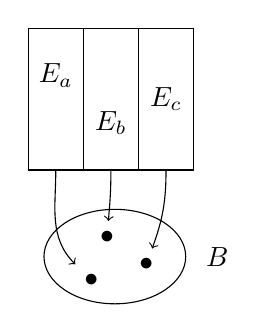
\begin{tikzpicture}
\draw (2,0) ellipse (0.9 and 0.6);
\node at (3.3,0) {\(B\)};
\node (C) at (2.4,-0.1) {\(\bullet\)};
\node (D) at (1.7,-0.3) {\(\bullet\)};
\node (E) at (1.9,0.25) {\(\bullet\)};

\draw (0.9,1.1) rectangle (1.6,2.9);
\node (Do) at (1.25, 2.3) {\(E_a\)};
\draw (1.6,1.1) rectangle (2.3,2.9);
\node (Eo) at (1.95, 1.7) {\(E_b\)};
\draw (2.3,1.1) rectangle (3,2.9);
\node (Co) at (2.65, 2) {\(E_c\)};
\draw (1.25,1.1) edge[->, out=-90] (D);
\draw (1.95,1.1) edge[->, out=-90, in=85] (E);
\draw (2.65,1.1) edge[->, out=-90, in=70] (C);
\end{tikzpicture}
\end{center}

再如, 向量丛理应是依赖于流形上一点 \(x \in M\) 的向量空间 \(V(x)\),
但我们改将其定义为流形之间的连续映射 \(p : E \to M\).
这种技术在代数几何中达到巅峰, 以 Grothendieck 的相对视角
(relative point of view) 为典型.
例如希望表达每个 \(A(x)\) 都是紧空间, 则说 \(p\) 是紧合映射;
希望表达每个 \(A(x)\) 都是仿射空间, 则说 \(p\) 是仿射映射.%
\footnote{一般来说, 在代数几何中也可以直接考虑前者, 即
要求 \(p^{-1}\{x\}\) 是仿射空间, 等等. 但是这样往往无法得到正确
的定义, 因为这样仅仅要求每个点处 \(A(x)\) 都满足条件,
并没有要求不同点之间要求的融洽性.}

然而, 想要将这类定义变为类型论中的模型时, 就会遇到严重的问题.
在原本的写法 \(A(x)\) 中, 若有函数 \(f : Y \to X\),
那么可以直接代入 \(A(f(y))\), 就得到依赖 \(y \in Y\) 的依值对象.
这样, 先代入 \(f : Y \to X\), 再代入 \(g : Z \to Y\),
与直接一次性代入 \(f \circ g\) 显然按定义是相同的,
都等于 \(A(f(g(z)))\).
然而, 如果使用 \(p : E \to X\) 的写法, 那么代入操作在
转换之后就得到拉回 \(p' : E \times_X Y \to Y\).
然而, 两次拉回与一次性拉回基本不会直接相等, 它们仅仅是同构.
这一现象在数学中很常见. 例如集合之间
\(A \times (B \times C) \ne (A \times B) \times C\),
因为前者的元素形如 \((a, (b, c))\), 而后者形如
\(((a, b), c)\), 显然不相等.
一个简单的想法是我们想办法商去一个等价关系, 使得它们相等.
这也是不可取的. 例如 \(A \times B\) 与 \(B \times A\) 是同构的,
但是如果我们将它们视作相同, 即令 \((a, b) = (b, a)\),
那么当 \(A = B = \mathbb{R}\) 时,
就有 \((1, 2) = (2, 1) \in \mathbb{R}^2\), 故 \(1 = 2\), 矛盾.

对此, 又能提出补救的办法.
第一个想法是试图证明在类型论中具体需要的相等关系里,
不会涉及上面提到的交换律这样有问题的情况.
再者, 可以给范畴添加一些与已有的对象同构的新对象,
这样不会改变范畴本身, 但是使得上面的商操作得以进行.
这些技巧统称为\textbf{融贯定理}.

由于这类问题在技术上比较复杂, 但是在直观上又应当总是成立,
在一般的研究中, 往往不愿在此事上花费过多笔墨.
因此往往有许多不同的办法定义类型论的模型,
有一些与数学中遇到的对象比较接近, 因此便于构造具体的模型,
但是不满足上面提到的严格等式;
另一些与类型论中的语法比较接近, 因此便于证明与类型论的关系,
但是自然的数学对象往往不构成这种模型.
这种情况可以画出图表, 从横线的上方到下方需要解决一个融贯问题:

\begin{center}
\begin{tikzpicture}
  \node at (-3, 2) {局部积闭范畴};
  \node at (-1.2, 2.6) {意象};
  \node at (0.4, 0.8) {概括范畴};
  \node at (3, 1.6) {形式丛范畴};
  \draw (-5, 0) -- (5, 0);
  \node at (-2.9, -1) {具族范畴};
  \node at (-2.9, -1.5) {自然模型};
  \node at (-0.3, -1.9) {具集范畴};
  \node at (2.7, -0.7) {分裂概括范畴};
\end{tikzpicture}
\end{center}

% LCCC/topos, compcat, display map cat

% CwF (NatMod), CwA, split compcat

\section{范畴语义的历史} 

% 在 1984 年, Seely~\cite{seely:1984:lccc} 提出了依值类型与范畴论的一种对应关系.

\begin{itemize}
\item 1984 年, Seely~\cite{seely:1984:lccc}
首次具体写出了用丛表示依值类型, 拉回表示代换的思想.
这隐含了融贯问题, 稍后会介绍.
\item 1986 年, Cartmell~\cite{cartmell:1986:contextualcat}
提出了具集范畴 (category with attributes) 及有语境性的变体.
\item 1993 年, Bart Jacobs~\cite{jacobs:1993:comprehensioncat}
提出了概括范畴, 这统一了之前的诸多概念.
\item Curien~\cite{curien:1993:coherence} 与 Hofmann~\cite{hofmann:1995:lccccoh}
讨论了融贯问题, 并给出了解决方案.
\item 1995 年, Dybjer~\cite{dybjer:1995:internal}
为了在类型论内研究类型论, 提出了具族范畴 (category with families) 的概念.
\item 2014 年, Clairambault~\cite{clairambault:2014:biequivalence}
给出了融贯问题的完整答案, 这在 \cite{curien:2014:revisit} 中有总结.
\item 2015 年, 由 Voevodsky 的相关工作启发了
融贯问题的新解决方案~\cite{lumsdaine:2015:universes}, 这强调了宇宙的重要性.
\item 2018 年, 具族范畴被 Awodey~\cite{awodey:2018:natural} 和 Fiore 各自独立重新表述为自然模型.
\item 2019 年, 上村太一~\cite{uemura:2019:general}
提出了通用的框架, 给出了一大类类型论的语法与语义的关系.
\end{itemize}

\section{意象与内语言}\label{category:inner}

(less material)

list some concrete biequivalences

